\chapter{Expectations and Bounds}

The concept of expectation, has now been introduced in the context of discrete and continuous random variables.
We know from our previous discussion that expectations provide an effective way to summarize the information contained in the distribution of a random variable.
As we will see shortly, expectations are also very valuable in establishing bounds on probabilities.


\section{Moment Generating Functions}

The \emph{moment generating function} of a random variable $X$ is defined by
\begin{equation*}
M_X (s) = \Expect \left[ e^{s X} \right] .
\end{equation*}
For continuous random variables, the moment generating function becomes
\begin{equation*}
M_X (s) = \int_{-\infty}^{\infty} f_X (u) e^{s u} du .
\end{equation*}
The experienced reader will quickly recognize the definition of $M_X(s)$ as a variant of the \emph{Laplace Transform}, a widely used linear operator.
The moment generating function gets its name from the following property.
Suppose that $M_X(s)$ exists within an open interval around $s = 0$, then the $n$th moment of $X$ is given by
\begin{equation*}
\begin{split}
\frac{d^n}{ds^n} M_X (s) \Big|_{s=0}
&= \frac{d^n}{ds^n} \Expect \left[ e^{s X} \right] \Big|_{s=0}
= \Expect \left[ \frac{d^n}{ds^n} e^{s X} \right] \bigg|_{s=0} \\
&= \Expect \left[ X^n e^{s X} \right] \Big|_{s=0}
= \Expect [X^n] .
\end{split}
\end{equation*}
In words, if we differentiate $M_X(s)$ a total of $n$ times and then evaluate the resulting function at zero, we obtain the $n$th moment of $X$.
In particular, we have $\frac{d M_X}{ds}(0) = \Expect [X]$ and $\frac{d^2 M_X}{ds^2}(0) = \Expect [X^2]$.

\begin{example}[Exponential Random Variable]
Let $X$ be an exponential random variable with parameter $\lambda$.
The moment-generating function of $X$ is given by
\begin{equation*}
M_X (s) = \int_0^{\infty} \lambda e^{-\lambda u} e^{su} du
= \int_0^{\infty} \lambda e^{-(\lambda-s) u} du
= \frac{\lambda}{\lambda - s} .
\end{equation*}
The mean of $X$ is
\begin{equation*}
\Expect [X] = \frac{d M_X }{ds} (0)
= \left. \frac{\lambda}{(\lambda - s)^2} \right|_{s=0}
= \frac{1}{\lambda} ;
\end{equation*}
more generally, the $n$th moment of $X$ can be computed as
\begin{equation*}
\Expect [X^n] = \frac{d^n M_X }{ds^n} (0)
= \left. \frac{n! \lambda}{(\lambda - s)^{n+1}} \right|_{s=0}
= \frac{n!}{\lambda^n} .
\end{equation*}
Incidentally, we can deduce from these results that the variance of $X$ is $1/\lambda^2$.
\end{example}

The definition of the moment generating function applies to discrete random variables as well.
In fact, for integer-valued random variables, the moment generating function and the ordinary generating function are related through the equation \index{Ordinary generating function} \index{Moment generating function}
\begin{equation*}
M_X (s) = \sum_{k \in X(\Omega)} e^{sk} p_X(k) = G_X (e^s) .
\end{equation*}

\begin{example}[Discrete Uniform Random Variable]
Suppose $U$ is a discrete uniform random variable taking value in $U(\Omega) = \{ 1, 2, \ldots, n \}$.
Then, $p_U(k) = 1/n$ for $1 \leq k \leq n$ and
\begin{equation*}
M_U(s) = \sum_{k = 1}^n \frac{1}{n} e^{sk}
= \frac{1}{n} \sum_{k = 1}^n e^{sk}
= \frac {e^s (e^{ns} - 1)} {n (e^s - 1)} .
\end{equation*}
The moment generating function provides an alternate and somewhat intricate way to compute the mean of $U$,
\begin{equation*}
\begin{split}
\Expect [U] &= \frac{d M_U}{ds} (0)
= \lim_{s \rightarrow 0}
\frac{n e^{(n+2)s} - (n+1) e^{(n+1)s} + e^s}{n \left( e^s - 1 \right)^2} \\
&= \lim_{s \rightarrow 0}
\frac{n(n+2) e^{(n+1)s} - (n+1)^2 e^{ns} + 1}{2n \left( e^s - 1 \right)} \\
&= \lim_{s \rightarrow 0}
\frac{n(n+1)(n+2)n e^{(n+1)s} - n (n+1)^2 e^{ns}}{2n e^s}
= \frac {n + 1}{2} .
\end{split}
\end{equation*}
Notice the double application of \emph{l'H\^{o}pital's rule} to evaluate the derivative of $M_U(s)$ at zero.
This may be deemed a more contrived method to derive the expected value of a discrete uniform random variables, but it does not rely on prior knowledge of special sums.
Through similar steps, one can derive the second moment of $U$, which is equal to
\begin{equation*}
\Expect \left[ U^2 \right] = \frac{(n+1)(2n+1)}{6} .
\end{equation*}
From these two results, we can show that the variance of $U$ is $(n^2 - 1)/12$.
\end{example}

The simple form of the moment generating function of a standard normal random variable points to its importance in many situations.
The exponential function is analytic and possesses many representations.

\begin{example}[Gaussian Random Variable]
Let $X$ be a standard normal random variable whose PDF is given by
\begin{equation*}
f_X (u) = \frac{1}{\sqrt{2 \pi}} e^{- \frac{u^2}{2}}.
\end{equation*}
The moment generating function of $X$ is equal to
\begin{equation*}
\begin{split}
M_X (s) &= \Expect \left[ e^{sX} \right]
= \int_{- \infty}^{\infty} \frac{1}{\sqrt{2 \pi}} e^{- \frac{u^2}{2}} e^{su} du \\
&= \int_{- \infty}^{\infty} \frac{1}{\sqrt{2 \pi}} e^{- \frac{u^2 + 2 s u}{2}} du
= e^{\frac{s^2}{2}} \int_{- \infty}^{\infty}
\frac{1}{\sqrt{2 \pi}} e^{- \frac{u^2 - 2 s u + s^2}{2}} du \\
&= e^{\frac{s^2}{2}} \int_{- \infty}^{\infty}
\frac{1}{\sqrt{2 \pi}} e^{- \frac{(u - s)^2}{2}} du
= e^{\frac{s^2}{2}} .
\end{split}
\end{equation*}
The last equality follows from the normalization condition and the fact that the integrand is a Gaussian PDF.
\end{example}

Let $M_X(s)$ be the moment generating function associated with a random variable $X$, and consider the random variable $Y = aX + b$ where $a$ and $b$ are constant.
The moment generating function of $Y$ can be obtained as follows,
\begin{equation*}
M_Y (s) = \Expect \left[ e^{s X} \right]
= \Expect \left[ e^{s (aX + b)} \right]
= e^{sb} \Expect \left[ e^{saX} \right]
= e^{sb} M_X (as) .
\end{equation*}
Thus, if $Y$ is an affine function of $X$ then $M_Y (s) = e^{sb} M_X (as)$.

\begin{example}
We can use this property to identify the moment generating function of a Gaussian random variable with parameters $m$ and $\sigma^2$.
Recall that an affine function of a Gaussian random variable is also Gaussian.
Let $Y = \sigma X + m$, then the moment generating function of $Y$ becomes
\begin{equation*}
M_Y (s) = \Expect \left[ e^{sY} \right]
= \Expect \left[ e^{s(\sigma X + m)} \right]
= e^{sm} \Expect \left[ e^{s\sigma X} \right]
= e^{sm + \frac{s^2 \sigma^2}{2} } .
\end{equation*}
From this moment generating function, we get
\begin{align*}
\Expect [Y] &= \frac{d M_Y}{ds} (0)
= \left. \left[ \left(m + s \sigma^2 \right)
e^{sm + \frac{s^2 \sigma^2}{2} } \right] \right|_{s=0} = m \\
\begin{split}
\Expect \left[ Y^2 \right] &= \frac{d^2 M_Y}{ds^2} (0)
= \left.  \left[ \sigma^2 e^{sm + \frac{s^2 \sigma^2}{2} }
+ \left(m + s \sigma^2 \right)^2  e^{sm + \frac{s^2 \sigma^2}{2} } \right]
\right|_{s=0} \\
&= \sigma^2 + m^2 .
\end{split}
\end{align*}
The mean of $Y$ is $m$ and its variance is equal to $\sigma^2$, as anticipated.
\end{example}


\section{Important Inequalities}

There are many situations for which computing the exact value of a probability is impossible or impractical.
In such cases, it may be acceptable to provide bounds on the value of an elusive probability.
The expectation is most important in finding pertinent bounds.

As we will see, many upper bounds rely on the concept of dominating functions.
Suppose that $g(x)$ and $h(x)$ are two nonnegative function such that $g(x) \leq h(x)$ for all $x \in \RealNumbers$.
Then, for any continuous random variable $X$, the following inequality holds
\begin{equation*}
\begin{split}
\Expect [g(X)] &= \int_{-\infty}^{\infty} g(x) f_X(x) dx \\
&\leq \int_{-\infty}^{\infty} h(x) f_X (x) dx
= \Expect [h(X)] .
\end{split}
\end{equation*}
This is illustrated in Figure~\ref{figure:DominatingFcn}.
In words, the weighted integral of $g(\cdot)$ is dominated by the weighted integral of $h(\cdot)$, where $f_X (\cdot)$ acts as the weighting function.
This notion is instrumental in understanding bounding techniques.
\begin{figure}[thb]
\begin{center}
\begin{psfrags}
\psfrag{Y}[c]{$\RealNumbers$}
\psfrag{X}[c]{$\RealNumbers$}
\psfrag{h}[c]{$h(x)$}
\psfrag{g}[c]{$g(x)$}
\includegraphics[width=6.5cm]{Figures/10Chapter/DominatingFcn}
\end{psfrags}
\caption{If $g(x)$ and $h(x)$ are two nonnegative functions such that $g(x) \leq h(x)$ for all $x \in \RealNumbers$, then $\Expect [g (X)]$ is less than or equal to $\Expect [h(X)]$.}
\label{figure:DominatingFcn}
\end{center}
\end{figure}


\subsection{The Markov Inequality}

We begin our exposition of classical upper bounds with a result known as the \emph{Markov inequality}. \index{Markov inequality}
Recall that, for admissible set $S \subset \RealNumbers$, we have
\begin{equation*}
\Pr (X \in S) = \Expect \left[ \IndicatorFcn_S (X) \right] .
\end{equation*}
Thus, to obtain a bound on $\Pr (X \in S)$, it suffices to find a function that dominates $\IndicatorFcn_S (\cdot)$ and for which we can compute the expectation.

Suppose that we wish to bound $\Pr (X \geq a)$ where $X$ is a nonnegative random variable and $a > 0$.
In this case, we can select $S = [a, \infty)$ and function $h(x) = x/a$.
For any $x \geq 0$, we have $h(x) \geq \IndicatorFcn_S(x)$, as illustrated in Figure~\ref{figure:MarkovInequality}.
It follows that
\begin{equation*}
\Pr (X \geq a) = \Expect \left[ \IndicatorFcn_S(X) \right] \leq \frac{\Expect [X]}{a} .
\end{equation*}

\begin{figure}[thb]
\begin{center}
\begin{psfrags}
\psfrag{Y}[c]{$\RealNumbers$}
\psfrag{X}[c]{$\RealNumbers$}
\psfrag{h}[l]{$h(x) = \frac{x}{a}$}
\psfrag{g}[l]{$g(x) = \IndicatorFcn_S (x)$}
\psfrag{a}[c]{$a$}
\includegraphics[width=6.5cm]{Figures/10Chapter/Markov}
\end{psfrags}
\caption{Suppose that we wish to find a bound for $\Pr (X \leq a)$.
We define set $S = [a, \infty)$ and function $g(x) = \IndicatorFcn_S (x)$.
Using dominating function $h(x) = x/a$, we conclude that $\Pr(X \geq a) \leq a^{-1} \Expect [X]$ for any nonnegative random variable $X$.}
\label{figure:MarkovInequality}
\end{center}
\end{figure}


\subsection{The Chebyshev Inequality}

The \emph{Chebyshev inequality} provides an extension to this methodology to various dominating functions. \index{Chebyshev inequality}
This yields a number of bounds that become useful in a myriad of contexts.

\begin{proposition}[Chebyshev Inequality]
Suppose $h (\cdot)$ is a nonnegative function and let $S$ be an admissible set.
We denote the infimum of $h (\cdot)$ over $S$ by
\begin{equation*}
i_S = \inf_{ x \in S } h (x) .
\end{equation*}
The Chebyshev inequality asserts that
\begin{equation} \label{equation:ChebyshevInequality}
i_S \Pr (X \in S)
\leq \Expect [ h(X) ]
\end{equation}
where $X$ is an arbitrary random variable.
\end{proposition}
\begin{proof}
This is a remarkably powerful result and it can be shown in a few steps.
The definition of $i_S$ and the fact that $h (\cdot)$ is nonnegative imply that
\begin{equation*}
i_S \IndicatorFcn_S (x) \leq h(x) \IndicatorFcn_S (x) \leq h(x)
\end{equation*}
for any $x \in \RealNumbers$.
Moreover, for any such $x$ and distribution $f_X(\cdot)$, we can write $i_S \IndicatorFcn_S (x) f_X(x) \leq h(x) f(x)$, which in turn yields
\begin{equation*}
\begin{split}
i_S \Pr (X \in S) &= \Expect \left[ i_s \IndicatorFcn_S (X) \right]
= \int_{\RealNumbers} i_S \IndicatorFcn_S (u) f_X(u) du \\
&\leq \int_{\RealNumbers} h (u) f_X(u) du
= \Expect [ h(X) ] .
\end{split}
\end{equation*}
When $i_S > 0$, this provides the upper bound $\Pr (X \in S) \leq i_S^{-1} \Expect [h (X)]$.
\end{proof}

Although the proof assumes a continuous random variable, we emphasize that the Chebyshev inequality applies to both discrete and continuous random variables alike.
The interested reader can rework the proof using the discrete setting and a generic PMF.
We provide special instances of the Chebyshev inequality below.

\begin{example}
Consider the nonnegative function $h(x) = x^2$ and let $S = \{ x | x^2 \geq b^2 \}$ where $b$ is a positive constant.
We wish to find a bound on the probability that $|X|$ exceeds $b$.
Using the Chebyshev inequality, we have $i_S = \inf_{x \in S} x^2 = b^2$ and, consequently, we get
\begin{equation*}
b^2 \Pr (X \in S) \leq \Expect \left[ X^2 \right] .
\end{equation*}
Constant $b$ being a positive real number, we can rewrite this equation as
\begin{equation*}
\Pr (|X| \geq b) = \Pr (X \in S) \leq \frac{\Expect \left[ X^2 \right]}{b^2} .
\end{equation*}
\end{example}

\begin{example}[The Cantelli Inequality]
Suppose that $X$ is a random variable with mean $m$ and variance $\sigma^2$.
We wish to show that
\begin{equation*}
\Pr ( X - m \geq a ) \leq \frac{\sigma^2}{a^2 + \sigma^2},
\end{equation*}
where $a \geq 0$.

This equation is slightly more involved and requires a small optimization in addition to the Chebyshev inequality.
Define $Y = X - m$ and note that, by construction, we have $\Expect [Y] = 0$.
Consider the probability $\Pr (Y \geq a)$ where $a > 0$, and let $S = \{ y | y \geq a \}$.
Also, define the nonnegative function $h(y) = (y + b)^2$, where $b > 0$.
Following the steps of the Chebyshev inequality, we write the infimum of $h(y)$ over $S$ as
\begin{equation*}
i_S = \inf_{y \in S} (y + b)^2 = (a + b)^2 .
\end{equation*}
Then, applying the Chebyshev inequality, we obtain
\begin{equation} \label{equation:CantelliProof}
\Pr (Y \geq a) \leq \frac{ \Expect \left[ (Y + b)^2 \right] }{(a + b)^2}
= \frac{ \sigma^2 + b^2 }{ (a + b)^2 } .
\end{equation}
This inequality holds for any $b > 0$.
To produce a better upper bound, we minimize the right-hand side of \eqref{equation:CantelliProof} over all possible values of $b$.
Differentiating this expression and setting the derivative equal to zero yields
\begin{equation*}
\frac{ 2 b }{(a + b)^2 } = \frac{ 2 \left( \sigma^2 + b^2 \right) }{(a + b)^3}
\end{equation*}
or, equivalently, $b = \sigma^2 / a$.
A second derivative test reveals that this is indeed a minimum.
Collecting these results, we obtain
\begin{equation*}
\Pr (Y \geq a) \leq \frac{ \sigma^2 + b^2 }{ (a + b)^2 }
%= \frac{ \sigma^2 + \sigma^4/a^2 }{ (a + \sigma^2/a)^2 }
%= \frac{ \sigma^2 (a^2 + \sigma^2) }{ (a^2 + \sigma^2)^2 }
= \frac{ \sigma^2 }{ a^2 + \sigma^2 } .
\end{equation*}
Substituting $Y = X - m$ leads to the desired result.
\end{example}

In some circumstances, a Chebyshev inequality can be tight.

\begin{example}
Let $a$ and $b$ be two constants such that $0 < b \leq a$.
Consider the function $h(x) = x^2$ along with the set $S = \{ x | x^2 \geq a^2 \}$.
Furthermore, let $X$ be a discrete random variable with PMF
\begin{equation*}
p_X (x) = \begin{cases} 1 - \frac{b^2}{a^2}, & x = 0 \\
\frac{b^2}{a^2}, & x = a \\
0, & \text{otherwise}. \end{cases}
\end{equation*}
For this random variable, we have $\Pr (X \in S) = b^2/a^2$.
By inspection, we also gather that the second moment of $X$ is equal to $\Expect \left[ X^2 \right] = b^2$.
Applying the Chebyshev inequality, we get $i_S = \inf_{x \in S} h(x) = a^2$ and therefore
\begin{equation*}
\Pr (X \in S) \leq i_S^{-1} \Expect \left[ h(X) \right]
= \frac{b^2}{a^2} .
\end{equation*}
Thus, in this particular example, the inequality is met with equality.
\end{example}


\subsection{The Chernoff Bound}

The \emph{Chernoff bound} is yet another upper bound that can be constructed from the Chebyshev inequality. \index{Chernoff bound}
Still, because of its central role in many application domains, it deserves its own section.
Suppose that we want to find a bound on the probability $\Pr (X \geq a)$.
We can apply the Chebyshev inequality using the nonnegative function $h(x) = e^{sx}$, where $s > 0$.
For this specific construction, $S = [a, \infty)$ and
\begin{equation*}
i_S = \inf_{x \in S} e^{sx} = e^{sa} .
\end{equation*}
It follows that
\begin{equation*}
\Pr (X \geq a) \leq e^{-sa} \Expect[ e^{sX} ] = e^{-sa} M_X(s) .
\end{equation*}
Because this inequality holds for any $s > 0$, we can optimize the upper bound over all possible values of $s$, thereby picking the best one,
\begin{equation} \label{equation:ChernoffBound}
\Pr (X \geq a) \leq \inf_{s > 0} e^{-sa} M_X(s) .
\end{equation}
This inequality is called the Chernoff bound.
It is sometimes expressed in terms of the log-moment generating function $\Lambda (s) = \log M_X (s)$.
In this latter case, \eqref{equation:ChernoffBound} translates into
\begin{equation} \label{equation:LogChernoffBound}
\log \Pr (X \geq a) \leq - \sup_{s > 0} \left\{ sa - \Lambda (s) \right\} .
\end{equation}
The right-hand side of \eqref{equation:LogChernoffBound} is called the \emph{Legendre transformation} of $\Lambda (s)$. \index{Legendre transformation}
Figure~\ref{figure:ChernoffBound} plots $e^{s(x-a)}$ for various values of $s > 0$.
It should be noted that all these functions dominate $\IndicatorFcn_{[a, \infty)}(x)$, and therefore they each provide a different bound on $\Pr (X \geq a)$.
It is natural to select the function that provides the best bound.
Yet, in general, this optimal $e^{s(x-a)}$ may depend on the distribution of $X$ and the value of $a$, which explains why \eqref{equation:ChernoffBound} involves a search over all possible values of $s$.

\begin{figure}[ht]
\begin{center}
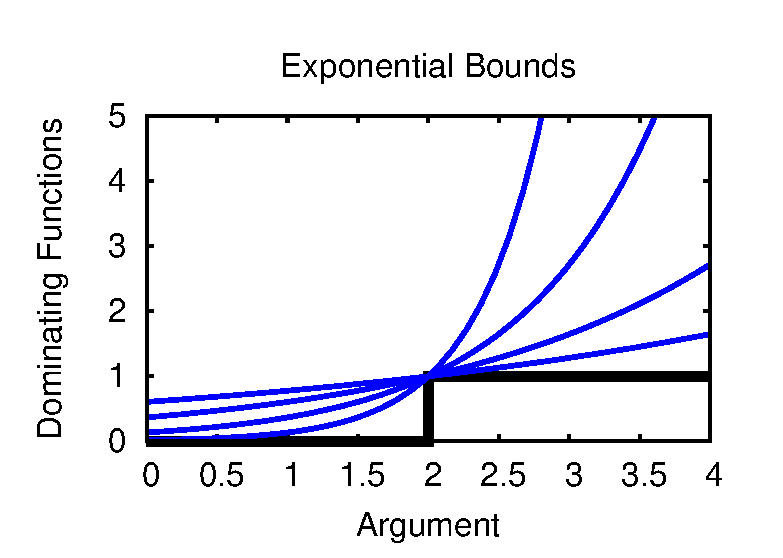
\includegraphics[width=8.5cm]{Figures/10chapter/chernoff_bound}
\end{center}
\caption{This figure illustrates how exponential functions can be employed to provide bounds on $\Pr (X > a)$.
Optimizing over all admissible exponential functions, $e^{s(x-a)}$ where $s > 0$, leads to the celebrated Chernoff bound.}
\label{figure:ChernoffBound}
\end{figure}


\subsection{Jensen's Inequality}

Some inequalities can be derived based on the properties of a single function.
The \emph{Jensen inequality} is one such example. \index{Jensen inequality}
Suppose that function $g(\cdot)$ is convex and twice differentiable, with
\begin{equation*}
\frac{d^2 g}{dx^2} (x) \geq 0
\end{equation*}
for all $x \in \RealNumbers$.
From the fundamental theorem of calculus, we have
\begin{equation*}
g(x) = g(a) + \int_a^x \frac{dg}{dx} (u) du .
\end{equation*}
Futhermore, because the second derivative of $g(\cdot)$ is a non-negative function, we gather that $\frac{dg}{dx} (\cdot)$ is a monotone increasing function.
As such, for any value of $a$, we have
\begin{equation*}
\begin{split}
g(x) &= g(a) + \int_a^x \frac{dg}{dx} (u) du \\
&\geq g(a) + \int_a^x \frac{dg}{dx} (a) du
= g(a) + (x-a) \frac{dg}{dx} (a) .
\end{split}
\end{equation*}
For random variable $X$, we then have
\begin{equation*}
g(X) \geq g(a) + (X-a) \frac{dg}{dx} (a) .
\end{equation*}
Choosing $a = \Expect [X]$ and taking expectations on both sides, we obtain
\begin{equation*}
\Expect [g(X)] \geq g(\Expect [X])
+ (\Expect [X]-\Expect [X]) \frac{dg}{dx} (\Expect [X])
= g(\Expect [X]) .
\end{equation*}
That is, $\Expect [g(X)] \geq g(\Expect [X])$, provided that these two expectations exist.
The Jensen inequality actually holds for convex functions that are not twice differentiable, but the proof is much harder in the general setting.


\section*{Further Reading}

\begin{small}
\begin{enumerate}
\item Ross, S., \emph{A First Course in Probability}, 7th edition, Pearson Prentice Hall, 2006: Sections~5.2, 7.7, 8.2.
\item Bertsekas, D. P., and Tsitsiklis, J. N., \emph{Introduction to Probability}, Athena Scientific, 2002: Section~3.1, 4.1, 7.1.
\item Gubner, J. A., \emph{Probability and Random Processes for Electrical and Computer Engineers}, Cambridge, 2006: Sections~4.2--4.3.
\item Miller, S. L., and Childers, D. G., \emph{Probability and Random Processes with Applications to Signal Processing and Communications}, 2004: Section~5.2.
\end{enumerate}
\end{small}

